\documentclass{beamer}
% Use DS9 global theme (includes pgfplots for visualization)
\usepackage{../../../shared/templates/ds9_theme}
\usepackage{minted} % For code highlighting

% Title page configuration
\title[Floats, Memory and IO]{CS12 03}
\subtitle{Floating Point Numbers, Data Size, and Console IO}
\author[Mr. Gullo]{Mr. Gullo}
\date[Sep 3, 2025]{September 3, 2025}

\begin{document}

\frame{\titlepage}

\begin{frame}
\frametitle{Learning Objectives}
\begin{itemize}
    \item Understand and use the \texttt{float} data type for decimal numbers.
    \item Differentiate between integer division and floating-point division.
    \item Define the fundamental memory units: \alert{bit} and \alert{byte}.
    \item Use the \texttt{sizeof()} operator to determine the memory size of data types.
    \item Understand the basics of binary (base-2) numbers and their representation in C++.
    \item Get user input from the console using \texttt{cin}.
\end{itemize}
\end{frame}

\section{Floating-Point Numbers}

\begin{frame}[fragile]
\frametitle{The \texttt{float} Data Type}
\begin{itemize}
    \item In programming, numbers with decimal points are called \alert{floating-point numbers}.
    \item C++ provides the \texttt{float} and \texttt{double} data types to store these values.
    \item \texttt{double} has higher precision (more decimal places) than \texttt{float}.
\end{itemize}

\begin{block}{Declaration and Initialization}
\begin{minted}[fontsize=\small]{cpp}
float pi_approx = 3.14159;
double gravity = 9.81;
\end{minted}
\end{block}

\begin{itemize}
    \item Floats support the same operations as integers (+, -, *, /) except for the modulo operator (\%).
\end{itemize}
\end{frame}

\begin{frame}[fragile]
\frametitle{Integer vs. Floating-Point Division}
A critical concept in C++ is how the division operator \texttt{/} behaves.

\begin{columns}
\column{0.5\textwidth}
\begin{block}{Integer Division}
If \alert{both} operands are integers, the result is an integer. Any fractional part is \alert{truncated} (cut off).
\begin{minted}{cpp}
int result = 5 / 4;
// result is 1
\end{minted}
\end{block}

\column{0.5\textwidth}
\begin{block}{Floating-Point Division}
If \alert{at least one} operand is a float or double, the result is a float or double.
\begin{minted}{cpp}
float result = 5.0 / 4;
// result is 1.25
\end{minted}
\end{block}
\end{columns}
\end{frame}

\begin{frame}[fragile]
\frametitle{Code Example: Division in Action}
Let's examine a program that demonstrates this behavior.
\begin{minted}{cpp}
#include <iostream>

using namespace std;

int main()
{
   float a = 5;
   float b = 4;
   float c = 5/4; // Integer division happens first!

   cout << "5/4 = " << 5/4 << endl;
   cout << "c = " << c << endl;
   cout << "5.0/4 = " << 5.0/4 << endl;
   cout << "5/4.0 = " << 5/4.0 << endl;
   cout << "a/b = " << a/b << endl;

   return 0;
}
\end{minted}
\end{frame}

\begin{frame}[fragile]
\frametitle{Code Example: Division Output}
\begin{block}{Program Output}
\begin{verbatim}
5/4 = 1
c = 1
5.0/4 = 1.25
5/4.0 = 1.25
a/b = 1.25
\end{verbatim}
\end{block}

\begin{itemize}
    \item \texttt{5/4}: Both are integer literals, so integer division occurs. The result is 1.
    \item \texttt{c = 5/4}: The integer division `5/4` is performed first, resulting in `1`. Then, the integer `1` is stored in the float variable `c`.
    \item \texttt{5.0/4} and \texttt{5/4.0}: One operand is a floating-point literal, so floating-point division occurs.
    \item \texttt{a/b}: The variables `a` and `b` are floats, so floating-point division occurs.
\end{itemize}
\end{frame}

\section{Memory and Data Types}

\begin{frame}
\frametitle{Key Concepts: Bits and Bytes}
\begin{itemize}
    \item \alert{Bit}:
    \begin{itemize}
        \item Short for \textbf{Bi}nary Digi\textbf{t}.
        \item The smallest unit of data in a computer.
        \item Can hold one of two values: 0 or 1.
    \end{itemize}
    \bigskip
    \item \alert{Byte}:
    \begin{itemize}
        \item A group of \textbf{8 bits}.
        \item The fundamental addressable unit of memory.
        \item One byte can store a single character, like 'A' or '?'.
    \end{itemize}
\end{itemize}
\end{frame}

\begin{frame}
\frametitle{Concept Visualization: Bits in a Byte}
\begin{itemize}
    \item To understand memory, we can visualize how these fundamental units are related.
    \item A byte is simply a sequence of 8 bits. Each of these bits can be either a `0` or a `1`.
    \item The different combinations of these 8 bits allow us to represent numbers, letters, and symbols.
\end{itemize}
\end{frame}

\begin{frame}
\frametitle{Visualization: A Single Byte}
\centering
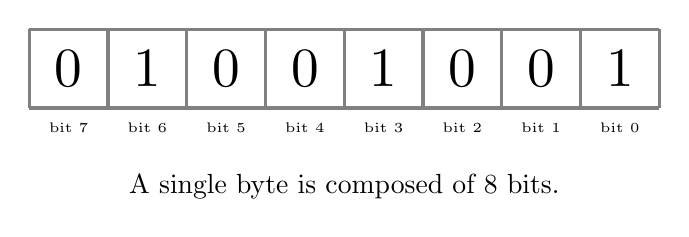
\begin{tikzpicture}[scale=1.0]
    % Draw the grid for the byte
    \draw[step=1cm, gray, very thick] (0,0) grid (8,1);
    
    % Add bit values
    \node[scale=2] at (0.5, 0.5) {0};
    \node[scale=2] at (1.5, 0.5) {1};
    \node[scale=2] at (2.5, 0.5) {0};
    \node[scale=2] at (3.5, 0.5) {0};
    \node[scale=2] at (4.5, 0.5) {1};
    \node[scale=2] at (5.5, 0.5) {0};
    \node[scale=2] at (6.5, 0.5) {0};
    \node[scale=2] at (7.5, 0.5) {1};
    
    % Add labels for bit positions
    \foreach \x in {0,...,7} {
        \node at (7.5-\x, -0.25) {\tiny bit \x};
    }
    
    \node at (4, -1) {A single byte is composed of 8 bits.};
\end{tikzpicture}
\end{frame}

\begin{frame}[fragile]
\frametitle{The \texttt{sizeof()} Operator}
\begin{itemize}
    \item Different data types require different amounts of memory.
    \item C++ provides the \texttt{sizeof()} operator to find out how many \alert{bytes} a data type or variable occupies in memory.
    \item This is a \textit{compile-time} operator, meaning the value is determined when you build your program, not when it runs.
\end{itemize}

\begin{block}{Syntax}
\begin{minted}{cpp}
cout << sizeof(int);      // Size of the int data type
int my_var = 10;
cout << sizeof(my_var);   // Size of the variable my_var
\end{minted}
\end{block}
\end{frame}

\begin{frame}[fragile]
\frametitle{Code Example: Finding Data Type Sizes}
This program neatly prints the memory size of common data types.
\begin{minted}[fontsize=\scriptsize]{cpp}
#include <iostream>

using namespace std;

int main()
{
    cout << "Integers:\n";
    cout << "Data Type    Bytes\n"
         << "-------------------\n"
         << "int           " << sizeof(int) << endl
         << "char          " << sizeof(char) << endl
         << "bool          " << sizeof(bool) << endl
         << "short int     " << sizeof(short) << endl << endl;

    cout << "Floating-Point:\n";
    cout << "Data Type    Bytes\n"
         << "-------------------\n"
         << "float         " << sizeof(float) << endl
         << "double        " << sizeof(double) << endl;

  return 0;
}
\end{minted}
\end{frame}

\begin{frame}[fragile]
\frametitle{Data Type Sizes: Output}
\begin{block}{Program Output (Typical)}
\begin{verbatim}
Integers:
Data Type    Bytes
-------------------
int           4
char          1
bool          1
short int     2

Floating-Point:
Data Type    Bytes
-------------------
float         4
double        8
\end{verbatim}
\end{block}
\note{Note: These sizes can vary depending on the system architecture (e.g., 32-bit vs 64-bit), but these are the most common values.}
\end{frame}

\section{Binary Numbers}

\begin{frame}
\frametitle{Concept: Binary (Base-2) System}
\begin{itemize}
    \item We normally use the \alert{decimal (base-10)} system, with digits 0-9.
    \item Computers use the \alert{binary (base-2)} system, with digits 0 and 1.
\end{itemize}
\begin{block}{Decimal Expansion}
$827_{10} = 8 \times 10^2 + 2 \times 10^1 + 7 \times 10^0$
\end{block}
\begin{block}{Binary Expansion}
$1011_2 = 1 \times 2^3 + 0 \times 2^2 + 1 \times 2^1 + 1 \times 2^0 = 8 + 0 + 2 + 1 = 11_{10}$
\end{block}
\end{frame}

\begin{frame}[fragile]
\frametitle{Binary Literals in C++}
\begin{itemize}
    \item You can write numbers in binary directly in your C++ code by using the prefix \texttt{0b}.
    \item When you print the number, C++ will display its decimal (base-10) equivalent by default.
\end{itemize}

\begin{block}{Code Example}
\begin{minted}{cpp}
#include <iostream>

int main()
{
    int binary_num = 0b1010011;
    std::cout << "0b1010011 = " << binary_num << std::endl;
    return 0;
}
\end{minted}
\end{block}

\begin{block}{Program Output}
\begin{verbatim}
0b1010011 = 83
\end{verbatim}
\end{block}
\end{frame}

\section{Console Input}

\begin{frame}[fragile]
\frametitle{Getting User Input with \texttt{cin}}
\begin{itemize}
    \item So far, our programs have had fixed values. To make them interactive, we need to get input from the user.
    \item C++ uses the \texttt{cin} object (part of \texttt{iostream}) for console input.
    \item The \alert{extraction operator \texttt{>>}} is used to "extract" data from the input stream and store it in a variable.
\end{itemize}

\begin{block}{Syntax}
\begin{minted}{cpp}
#include <iostream>
using namespace std;

int main() {
    int age;
    cout << "Please enter your age: ";
    cin >> age; // Waits for user input, then stores it in 'age'
    cout << "You are " << age << " years old." << endl;
    return 0;
}
\end{minted}
\end{block}
\end{frame}

\begin{frame}
\frametitle{I do: Find the $n^{th}$ Triangular Number}
\begin{block}{Problem}
Write a program that asks the user for a number, $n$, and calculates the $n^{th}$ triangular number. The formula is $t_n = \frac{n(n+1)}{2}$.
\end{block}

\begin{itemize}
    \item \textbf{G - Givens}: The user will provide an integer \texttt{n}. The formula is known.
    \item \textbf{U - Unknown}: The value of the $n^{th}$ triangular number.
    \item \textbf{E - Equation (Logic)}:
    \begin{enumerate}
        \item Prompt the user for a number.
        \item Declare an integer variable \texttt{n} to store the input.
        \item Use \texttt{cin >> n} to read the user's value.
        \item Calculate the result using the formula \texttt{n * (n + 1) / 2}.
        \item Print the formatted result to the console.
    \end{enumerate}
\end{itemize}
\end{frame}

\begin{frame}[fragile]
\frametitle{I do: Triangular Number Solution}
\begin{itemize}
    \item \textbf{S - Substitute (Code)}:
\end{itemize}
\begin{minted}{cpp}
#include <iostream>
using namespace std;

int main() {
    int n;
    cout << "What triangle number would you like to find? ";
    cin >> n;
    cout << "t_" << n << " = " << n * (n + 1) / 2 << endl;
    return 0;
}
\end{minted}
\begin{itemize}
    \item \textbf{S - Solve (Output)}:
\end{itemize}
\begin{block}{Sample Run}
\begin{verbatim}
What triangle number would you like to find? 17
t_17 = 153
\end{verbatim}
\end{block}
\end{frame}


\begin{frame}[fragile]
\frametitle{We do: Arithmetic Sequence}
\begin{block}{Problem}
Write a code chunk that prompts the user for $n$ then displays the $n^{th}$ number in the following arithmetic sequence: $11, 15, 19, 23, ...$
\end{block}

\begin{itemize}
    \item What is the common difference, $d$? \alert{4}
    \item What is the first term, $a_1$? \alert{11}
    \item What is the formula for the $n^{th}$ term? $a_n = a_1 + (n-1)d$
\end{itemize}

\begin{block}{Skeleton Code}
\begin{minted}{cpp}
// includes...
int n;
cout << "Enter a term number: ";
cin >> n;

int result = _______________; // What goes here?

cout << "The " << n << "th term is " << result << endl;
\end{minted}
\end{block}
\end{frame}

\begin{frame}
\frametitle{You do: Arithmetic Series Sum}
\begin{block}{Problem}
Write a C++ program that prompts the user for $n$ and then displays the \textbf{sum} of the first $n$ terms in the following arithmetic series:
$2 + 5 + 8 + 11 + ...$
\end{block}

\begin{alertblock}{Hint}
The formula for the sum of the first $n$ terms of an arithmetic series is:
$S_n = \frac{n}{2}(2a_1 + (n-1)d)$
\begin{itemize}
    \item $a_1$ is the first term.
    \item $d$ is the common difference.
\end{itemize}
\end{alertblock}

\begin{itemize}
    \item Use the problem-solving steps from our "I do" example to structure your code.
\end{itemize}
\end{frame}


\begin{frame}
\frametitle{Summary}
\begin{itemize}
    \item Use \texttt{float} or \texttt{double} for numbers with decimal points.
    \item Division with two integers (\texttt{int / int}) results in an \alert{integer} (truncation). To get a decimal result, ensure at least one operand is a float or double (\texttt{float / int}).
    \item A \alert{bit} is a 0 or 1. A \alert{byte} is 8 bits.
    \item The \texttt{sizeof()} operator tells you how many bytes a data type uses.
    \item Binary numbers (base-2) are fundamental to computing. In C++, use the \texttt{0b} prefix for binary literals (e.g., \texttt{0b1101}).
    \item Use \texttt{cin >> variable;} to get interactive input from the user.
\end{itemize}
\end{frame}

\end{document}